\section{Results}\label{sec:results}

\subsection{Spatial and Temporal Patterns}

Figure~\ref{fig:maps} maps the DFA and RCD indices for 2013 and 2021. Three patterns stand out. First, both indices increased over the sample period. The national average DFA rose from 0.109 in 2013 to 0.379 in 2021, and the average RCD rose from 0.298 to 0.520. The increase was not confined to a few leading provinces; most provinces moved into higher classes between 2013 and 2021.

Second, the spatial distribution is persistent. The eastern region has the highest DFA and RCD values throughout the period, followed by the central region, the northeastern region, and the western region. In 2021, the eastern averages were 0.406 for DFA and 0.557 for RCD, compared with 0.174 and 0.312 in the western region. The ranking of provinces is relatively stable, which is consistent with the view that digital and economic advantages are cumulative.

Third, the gap in DFA is larger than the gap in RCD. In 2013, the province with the highest DFA had a value more than 80 times that of the lowest, while the RCD range was much narrower. By 2021, the DFA gap had narrowed but remained substantial, whereas the RCD gap had changed less. This pattern suggests that digital factors diffuse faster than the broader conditions required for coordinated development, which motivates the threshold analysis below.

\begin{figure}[H]
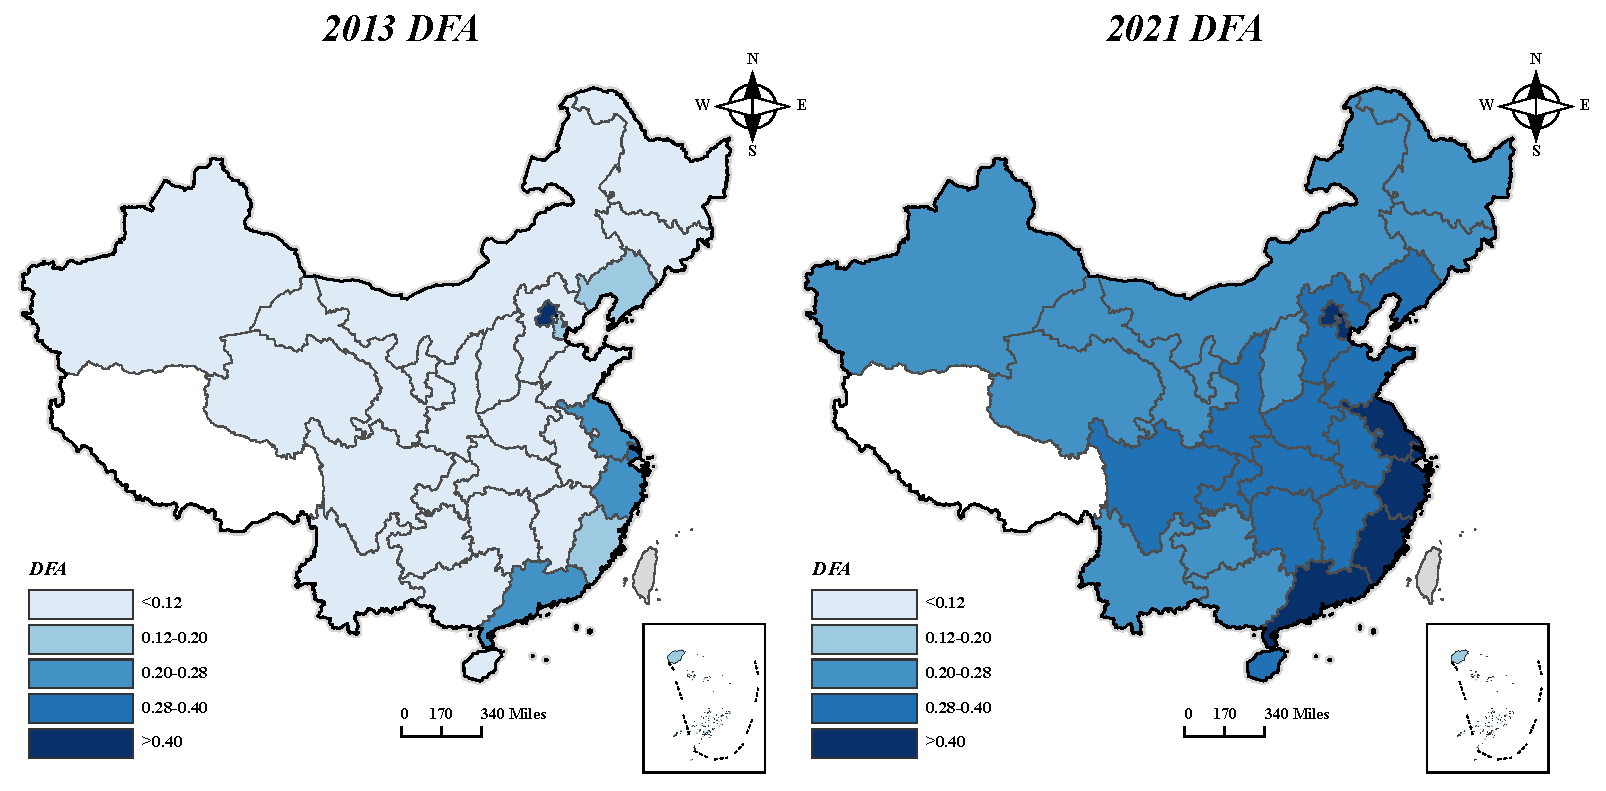
\includegraphics[width=\textwidth]{figures/fig2a_dfa_map_2p.pdf}\\[2pt]
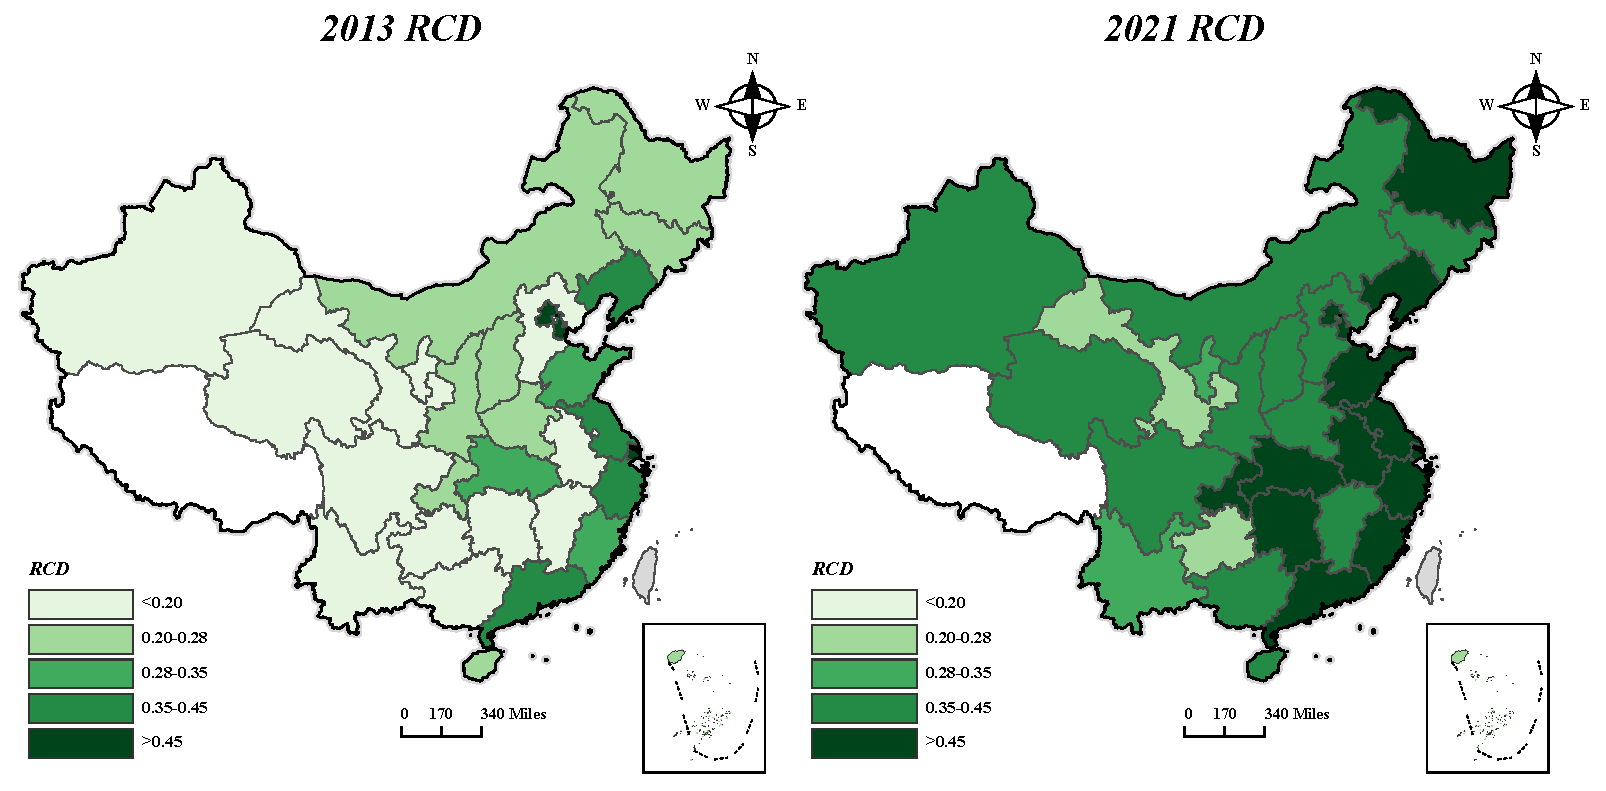
\includegraphics[width=\textwidth]{figures/fig2b_rcd_map_2p.pdf}
\caption{Spatial distribution of DFA and RCD, 2013 and 2021. (a) DFA; (b) RCD. Tibet is shown in white and Taiwan in light gray because they are not included in the estimation sample. The five classes use fixed cutoffs for comparability across years.}\label{fig:maps}
\end{figure}

Figure~\ref{fig:trends} shows the regional averages over time. The eastern region maintains a clear lead in both indices. The western region starts from the lowest level but grows faster in DFA, especially after 2015. The northeastern region has a relatively high initial RCD but a slow digital transition, and its RCD growth is modest. These regional trajectories are consistent with the heterogeneity analysis in Section~\ref{sec:heterogeneity}.

\begin{figure}[H]
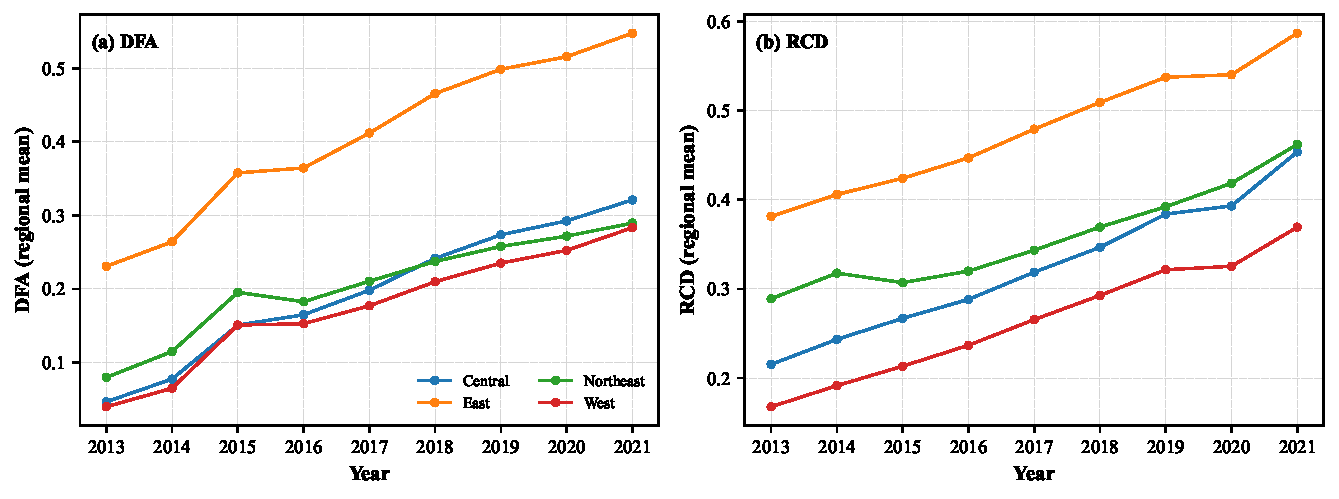
\includegraphics[width=\textwidth]{figures/fig6_trends.pdf}
\caption{Regional averages of DFA and RCD, 2013--2021. (a) DFA; (b) RCD. Regions are defined as East, Central, West, and Northeast.}\label{fig:trends}
\end{figure}

\subsection{Baseline Estimates}\label{sec:baseline}

Table~\ref{tab:baseline} reports the baseline estimates. Column (1) includes DFA without controls and with province and year fixed effects. The coefficient is 0.277 and is significant at the 5\% level. Column (2) adds the four controls. The coefficient falls to 0.241 but remains significant at the 5\% level. Column (3) adds region-specific linear trends to absorb differential regional trends. The coefficient is 0.204 and is significant at the 10\% level. Column (4) uses the five-dimension RCD index as the outcome; the coefficient is 0.013 and is not statistically significant.

The baseline estimate implies that a one-unit increase in the DFA index is associated with an increase of 0.241 points in the RCD index, or about 1.6 standard deviations of RCD. Since the DFA index ranges from 0 to 1, this is a large effect at the upper end of the distribution. A more modest increase of one standard deviation in DFA (0.179) is associated with an increase of about 0.043 points in RCD, or 0.29 standard deviations. The estimate is therefore economically meaningful as well as statistically significant.

The controls are generally insignificant. Government intervention, FDI, population density, and private economy vitality do not have robust associations with RCD once province and year fixed effects are included. This is not surprising: the controls are intended to absorb local conditions, not to explain RCD. Their inclusion does not change the DFA coefficient much, which suggests that the baseline result is not driven by these observable confounders.

The contrast between columns (2) and (4) is informative. DFA is positively associated with the three core coordination dimensions but not with the extended five-dimension index. The extended index adds infrastructure and ecological coordination, which are slower-moving and may respond to digitalization with a longer lag. The result suggests that the short-run effect of DFA operates mainly through economic, social, and urban-rural coordination, not through infrastructure or ecological outcomes. We return to this point in the robustness discussion.

\begin{table}[H]
\caption{Baseline estimates of the effect of DFA on RCD.}\label{tab:baseline}
\begin{threeparttable}
\small
\begin{tabular}{lrrrr}
\toprule
 & (1) & (2) & (3) & (4) \\
\midrule
DFA & 0.277** & 0.241** & 0.204* & 0.013 \\
 & (0.112) & (0.118) & (0.118) & (0.133) \\[2pt]
Government intervention &  & -0.0012 & -0.0007 & -0.0001 \\
 &  & (0.001) & (0.001) & (0.001) \\[2pt]
Log FDI &  & 0.0215 & 0.0169 & 0.0183 \\
 &  & (0.016) & (0.017) & (0.013) \\[2pt]
Log population density &  & 0.0794 & 0.1483 & 0.1003 \\
 &  & (0.138) & (0.203) & (0.129) \\[2pt]
Private economy &  & -0.00002 & 0.00011 & -0.00016 \\
 &  & (0.000) & (0.000) & (0.000) \\[2pt]
Controls & No & Yes & Yes & Yes \\
Province FE & Yes & Yes & Yes & Yes \\
Year FE & Yes & Yes & Yes & Yes \\
Region trends & No & No & Yes & No \\
Observations & 270 & 270 & 270 & 270 \\
\bottomrule
\end{tabular}
\begin{tablenotes}
\small
\item Notes: The dependent variable is RCD in columns (1)--(3) and RCD5 in column (4). DFA is the digital factor allocation index. Controls include government intervention, log FDI per capita, log population density, and private economy vitality. Province and year fixed effects are included in all columns. Region trends are region-specific linear trends. Standard errors clustered by province are in parentheses. $^{***}p<0.01$, $^{**}p<0.05$, $^{*}p<0.10$.
\end{tablenotes}
\end{threeparttable}
\end{table}

\subsection{Threshold Estimates}\label{sec:threshold}

Table~\ref{tab:threshold} reports the threshold tests and regime coefficients. Panel A shows the estimated threshold, the 95\% likelihood-ratio confidence interval, the $F$ statistic for the null of linearity, and the bootstrap $p$-value. Panel B shows the low- and high-regime coefficients of DFA.

The economic-development threshold is the main result. The estimated threshold is 10.589 in log GDP per capita, which corresponds to about CNY 39,700 per person. The bootstrap $p$-value is 0.003, so the null of linearity is rejected at the 1\% level. The low-regime coefficient is 0.506 and the high-regime coefficient is 0.677; both are significant at the 1\% level. The estimated marginal association is therefore about 34\% larger after economic development crosses the threshold. Because the threshold model absorbs only province fixed effects, its coefficients are not directly comparable to the two-way fixed-effects estimates in Table~\ref{tab:baseline}; the relevant comparison is between the low and high regimes within the threshold model. This pattern is consistent with H2 and with the absorptive-capacity interpretation: digital factor allocation is more effective when local income, markets, and complementary capabilities are sufficiently developed.

Figure~\ref{fig:lr} plots the likelihood-ratio statistic for the economic-development threshold. The minimum is sharp, and the 95\% confidence interval is narrow, ranging from 10.583 to 10.639. Figure~\ref{fig:scatter} shows the raw association between DFA and RCD, split by the threshold. The high-development regime has a steeper slope, although the raw scatter also reflects the strong cross-sectional correlation between the two indices. The threshold estimate is therefore best read together with the fixed-effects estimates in Table~\ref{tab:baseline}, which absorb time-invariant province characteristics.

\begin{table}[H]
\caption{Threshold tests and regime-specific coefficients.}\label{tab:threshold}
\begin{threeparttable}
\small
\textit{Panel A: Threshold tests}\\[2pt]
\begin{tabular}{lcccc}
\toprule
Threshold variable & $\hat{\gamma}$ & 95\% CI & $F$ & Bootstrap $p$ \\
\midrule
DFA & 0.178 & [0.153, 0.349] & 15.50 & 0.137 \\
ln(per capita GDP) & 10.589 & [10.583, 10.639] & 29.07 & 0.003 \\
Financial development & 10.045 & -- & 61.48 & 0.010 \\
Technological investment & 0.856 & [0.856, 0.998] & 22.70 & 0.120 \\
Private economy vitality & 368.402 & [85.480, 368.402] & 23.81 & 0.107 \\
\bottomrule
\end{tabular}\par\vspace{8pt}
\textit{Panel B: Regime-specific coefficients of DFA}\\[2pt]
\begin{tabular}{lccc}
\toprule
Threshold variable & Low regime & High regime & Observations (low/high) \\
\midrule
DFA & 0.549*** & 0.661*** & 90/180 \\
 & (0.060) & (0.066) & \\[2pt]
ln(per capita GDP) & 0.506*** & 0.677*** & 66/204 \\
 & (0.057) & (0.067) & \\[2pt]
Financial development & 0.578*** & 0.267*** & 240/30 \\
 & (0.065) & (0.082) & \\[2pt]
Technological investment & 0.812*** & 0.627*** & 33/237 \\
 & (0.088) & (0.051) & \\[2pt]
Private economy vitality & 0.652*** & 0.573*** & 244/26 \\
 & (0.066) & (0.070) & \\[2pt]
\bottomrule
\end{tabular}
\begin{tablenotes}
\small
\item Notes: Each row corresponds to a separate threshold model with province fixed effects and the full control set. The threshold is estimated by grid search over the inner 80\% of the threshold variable's distribution. The $F$ statistic tests the null of a single linear regime. The bootstrap $p$-value is based on 300 cluster wild bootstrap replications. Standard errors clustered by province are in parentheses. For financial development, the likelihood-ratio interval collapses at the grid resolution; it is therefore not reported. $^{***}p<0.01$, $^{**}p<0.05$, $^{*}p<0.10$.
\end{tablenotes}
\end{threeparttable}
\end{table}

\begin{figure}[H]
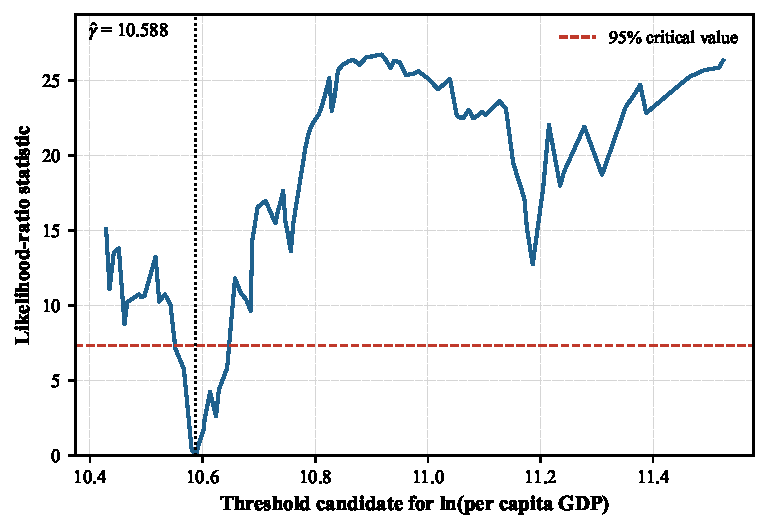
\includegraphics[width=0.68\textwidth]{figures/fig4_lr_curve.pdf}
\caption{Likelihood-ratio statistic for the economic-development threshold. The dashed line is the 95\% critical value (7.35). The dotted vertical line marks the estimated threshold.}\label{fig:lr}
\end{figure}

\begin{figure}[H]
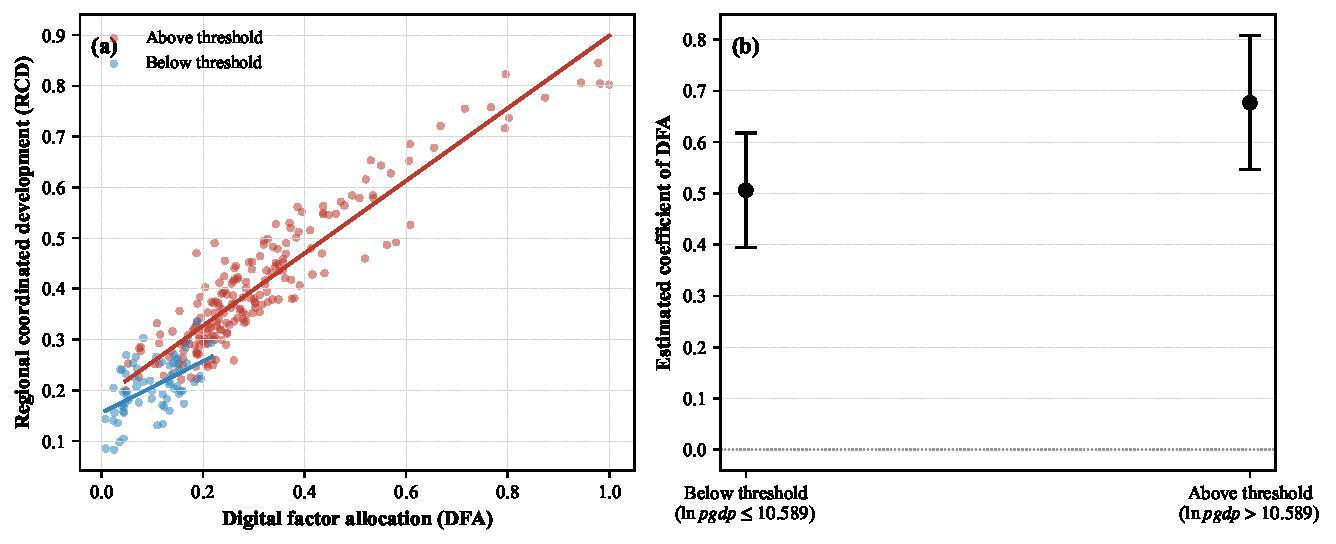
\includegraphics[width=\textwidth]{figures/fig3_scatter_regimes.pdf}
\caption{DFA, RCD, and the economic-development threshold. (a) Raw association between DFA and RCD, split by the estimated threshold; the lines are linear fits within each regime. (b) Regime-specific coefficients of DFA with 95\% confidence intervals from the threshold model.}\label{fig:scatter}
\end{figure}

The financial-development threshold is also statistically significant, but its interpretation requires caution. The estimated threshold is 10.045. The low-regime coefficient is 0.578 and the high-regime coefficient is 0.267; the bootstrap $p$-value is 0.010. The high regime contains 30 observations: 27 from Beijing, Shanghai, and Tianjin, plus three observations from Qinghai. The decline in the marginal effect is therefore driven by a small group of financially deep municipalities. It is consistent with diminishing returns to digital finance, but it should not be read as a general statement about all high-finance provinces.

The other threshold variables do not produce statistically significant breaks. The DFA self-threshold has a bootstrap $p$-value of 0.137, the technology threshold 0.120, and the private-economy threshold 0.107. The point estimates suggest some variation across regimes, but the null of linearity cannot be rejected. The nonlinearity in the data is therefore primarily associated with economic development, not with the level of digitalization itself.

One caveat applies to all threshold estimates. The threshold model follows Hansen (1999) and includes province fixed effects but not year fixed effects. Because the threshold variable is a slow-moving development indicator, year fixed effects would absorb much of the cross-province variation in development stages that identifies the threshold. When region-specific linear trends are added, the economic-development threshold remains positive but becomes statistically weaker (bootstrap $p=0.47$). The threshold should therefore be interpreted as a long-run structural pattern rather than a short-run causal effect. We discuss this limitation further in Section~\ref{sec:limitations}.

\subsection{Regional Heterogeneity}\label{sec:heterogeneity}

Table~\ref{tab:heterogeneity} reports the regional estimates. Under two-way fixed effects, the western region has a positive and highly significant coefficient of 0.555. The eastern and central coefficients are positive but insignificant (0.227 and 0.192), and the northeastern coefficient is negative and insignificant ($-0.223$). Under province fixed effects, all four regions have positive and significant coefficients, with the largest coefficients in the west (0.535) and central region (0.485), followed by the east (0.296) and the northeast (0.096).

The western result is the most robust. It holds under both specifications and is significant at the 1\% level. This is consistent with H4 and with the catch-up interpretation: the marginal return to digital factor allocation is higher in regions that start with lower levels of digital infrastructure and financial access. The eastern and central results are sensitive to the inclusion of year fixed effects, which suggests that their average association is partly driven by common national trends. The northeastern result is weak and sometimes negative, which may reflect the region's industrial legacy and slow digital transition.

The regional pattern should not be overinterpreted. The subsample estimates are less precise than the full-sample estimates, and the differences across regions are not formally tested. The results are best read as descriptive evidence that the DFA--RCD relationship is not uniform across China's regions, with the west showing the most consistent positive association.

\begin{table}[H]
\caption{Regional heterogeneity in the effect of DFA on RCD.}\label{tab:heterogeneity}
\begin{threeparttable}
\small
\begin{tabular}{lcc}
\toprule
Region & Two-way FE & Province FE \\
\midrule
East & 0.227 & 0.296*** \\
 & (0.234) & (0.104) \\[2pt]
Central & 0.192 & 0.485*** \\
 & (0.340) & (0.072) \\[2pt]
West & 0.555*** & 0.535*** \\
 & (0.125) & (0.077) \\[2pt]
Northeast & -0.223 & 0.096*** \\
 & (0.285) & (0.023) \\[2pt]
Controls & Yes & Yes \\
Observations & 90/54/99/27 & 90/54/99/27 \\
\bottomrule
\end{tabular}
\begin{tablenotes}
\small
\item Notes: Each cell reports the coefficient of DFA from a separate regression for the indicated region. Controls are included in all columns. Two-way FE includes province and year fixed effects; province FE includes province fixed effects only. Standard errors clustered by province are in parentheses. $^{***}p<0.01$, $^{**}p<0.05$, $^{*}p<0.10$.
\end{tablenotes}
\end{threeparttable}
\end{table}

\subsection{Robustness}\label{sec:robustness}

Table~\ref{tab:robustness} reports the robustness checks. The baseline coefficient is 0.241. It remains positive and significant when the RCD index is replaced by a globally entropy-weighted index (0.349), when the DFA index is replaced by an equal-weight indicator index (0.298), when municipalities are excluded (0.288), when the sample ends in 2019 (0.283), and when the outcome and regressor are winsorized at the 1st and 99th percentiles (0.302). The coefficient is larger under province fixed effects (0.689) and smaller and insignificant when the five-dimension RCD index, the coupling coordination degree, the entropy-weighted DFA index, or lagged DFA are used.

The pattern is informative. The positive effect is robust to alternative weighting of the RCD indicators and to the exclusion of the largest municipalities. It is also robust to dropping 2020, which suggests that the COVID-19 shock is not driving the result. The effect is weaker for the five-dimension RCD index and for the coupling coordination degree. This is consistent with the baseline contrast in Table~\ref{tab:baseline}: the five-dimension index adds infrastructure and ecological dimensions that are less responsive to DFA in the short run, and the coupling coordination degree emphasizes balance among dimensions rather than levels.

The insignificant coefficient for lagged DFA suggests that the effect is contemporaneous rather than delayed. This may reflect the fast diffusion of digital services: once infrastructure and platforms are available, their coordination effects appear within the same year. It may also reflect measurement: the DFA index captures the current state of digital factor allocation, and its effect on RCD is likely to be strongest when the digital environment is contemporaneous with economic and social outcomes.

The entropy-weighted DFA index produces a positive but insignificant coefficient. This index places more weight on IPv4 addresses and domain names, which are concentrated in a few leading provinces. The equal-weight index and the baseline index, which give more balanced weight to infrastructure, industry, finance, and human capital, produce stronger results. This suggests that the effect is not driven by a single digital indicator but by the combined allocation of digital factors.

\begin{table}[H]
\caption{Robustness checks.}\label{tab:robustness}
\begin{threeparttable}
\small
\begin{tabular}{lccc}
\toprule
Specification & Coefficient & SE & N \\
\midrule
Baseline & 0.241** & (0.118) & 270 \\
Five-dimension RCD & 0.013 & (0.133) & 270 \\
CCD of core dimensions & 0.118 & (0.288) & 270 \\
Entropy-weighted RCD & 0.349** & (0.154) & 270 \\
Equal-weight DFA & 0.298** & (0.143) & 270 \\
Entropy-weighted DFA & 0.186 & (0.176) & 270 \\
Excluding municipalities & 0.288** & (0.128) & 234 \\
2013-2019 & 0.283** & (0.123) & 210 \\
Additional controls & 0.213 & (0.138) & 270 \\
Province FE only & 0.689*** & (0.069) & 270 \\
Lagged DFA & 0.139 & (0.146) & 240 \\
Winsorized 1/99 & 0.302** & (0.122) & 270 \\
\bottomrule
\end{tabular}
\begin{tablenotes}
\small
\item Notes: Each row reports the coefficient of DFA (or lagged DFA) from a separate regression. The baseline includes the full control set and two-way fixed effects. The five-dimension RCD index adds infrastructure and ecological coordination. The coupling coordination degree is computed from the three core dimensions. The equal-weight DFA index uses equal weights for all 15 indicators. The entropy-weighted DFA index uses global entropy weights. The additional-controls specification adds technological investment, industrial structure upgrading, and financial development. Standard errors clustered by province are in parentheses. $^{***}p<0.01$, $^{**}p<0.05$, $^{*}p<0.10$.
\end{tablenotes}
\end{threeparttable}
\end{table}

\begin{figure}[H]
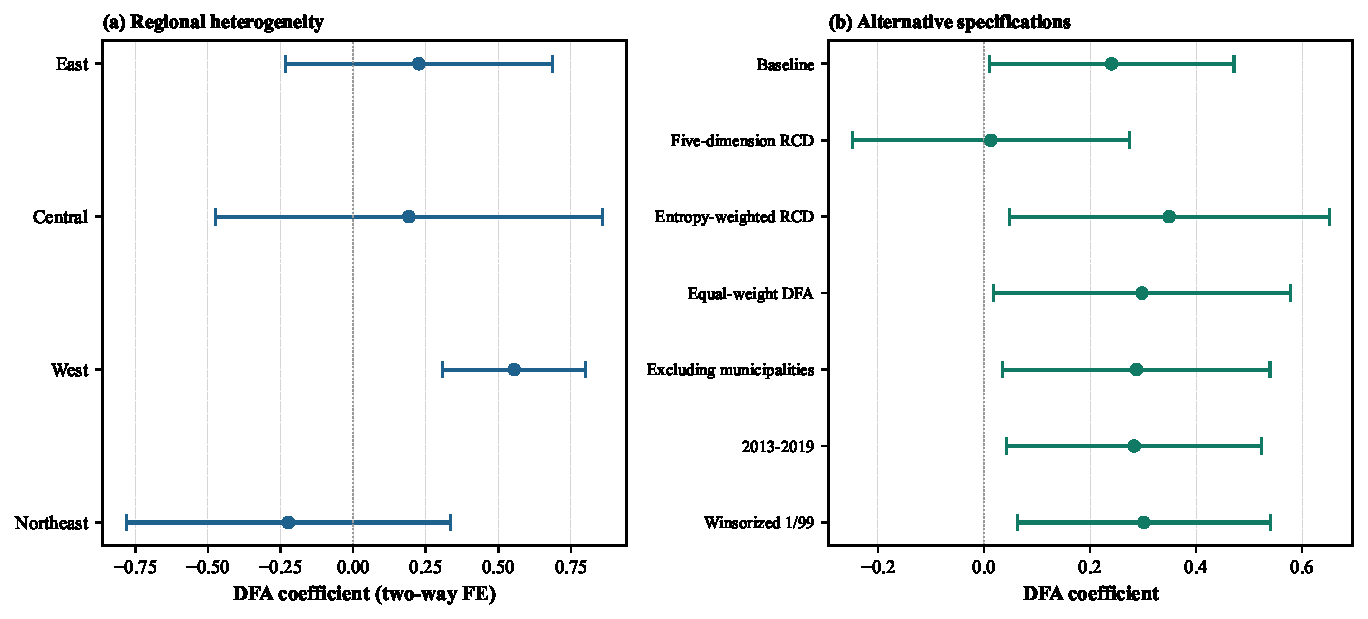
\includegraphics[width=\textwidth]{figures/fig5_coefficients.pdf}
\caption{Regional and specification heterogeneity. (a) Regional DFA coefficients under two-way fixed effects. (b) DFA coefficients under alternative specifications. Bars are 95\% confidence intervals.}\label{fig:coef}
\end{figure}

\subsection{Mechanisms}\label{sec:mechanisms}

Table~\ref{tab:mechanisms} reports the channel regressions. DFA is positively associated with technological investment (6.290, p < 0.05) and financial development (8.885, p < 0.01) under two-way fixed effects, and with industrial structure upgrading under province fixed effects (144.903, p < 0.01). These results are consistent with the view that digital factor allocation supports RCD through innovation, financial deepening, and structural change.

The income-gap result is more nuanced. Under two-way fixed effects, DFA is positively associated with the urban-rural income ratio (0.715, p < 0.05), which implies that a one-unit increase in DFA widens the urban-rural income gap in the short run. Under province fixed effects, the association is negative ($-1.279$, p < 0.01), which implies that over the longer run digital factor allocation is associated with a narrower gap. The contrast suggests that the distributional effect of digitalization is horizon-dependent: in the short run, digital opportunities may be captured disproportionately by urban and skilled groups, while in the longer run, the diffusion of digital services to rural areas may narrow the gap.

The mediator coefficients in the RCD equation are not statistically significant. This means that the channel evidence should be read as suggestive rather than as a formal mediation analysis. The reduced-form effect of DFA on RCD remains positive when the mediators are included, which suggests that the channels complement rather than fully explain the relationship. A more complete mediation analysis would require exogenous variation in each channel, which is beyond the scope of this study.

\begin{table}[H]
\caption{Channel regressions.}\label{tab:mechanisms}
\begin{threeparttable}
\small
\resizebox{\textwidth}{!}{\begin{tabular}{lccc}
\toprule
Mediator & DFA $\to$ M (two-way FE) & DFA $\to$ M (province FE) & M in RCD equation \\
\midrule
Technological investment & 6.290** & 1.255 & 0.006 \\
 & (2.985) & (1.275) & \\[2pt]
Financial development & 8.885*** & 4.941*** & -0.001 \\
 & (3.164) & (1.773) & \\[2pt]
Industrial upgrading & 127.226 & 144.903*** & -0.000 \\
 & (80.849) & (29.771) & \\[2pt]
Urban-rural income ratio & 0.715** & -1.279*** & -- \\
 & (0.302) & (0.180) & \\[2pt]
Controls & Yes & Yes & Yes \\
Observations & 270 & 270 & 270 \\
\bottomrule
\end{tabular}}
\begin{tablenotes}
\small
\item Notes: The first two columns report the effect of DFA on the mediator under two-way and province fixed effects, respectively. The third column reports the coefficient of the mediator in the RCD equation. Controls are included in all columns. Standard errors clustered by province are in parentheses. $^{***}p<0.01$, $^{**}p<0.05$, $^{*}p<0.10$.
\end{tablenotes}
\end{threeparttable}
\end{table}
